%
% tkz-euclide (14/01/2011)
%
% Coding (utf8) Creator (TeX) Producer (pdfeTeX)
% Author Alain Matthes
\input{tkzfctpreamble.ltx}

\begin{document}

 \begin{tikzpicture}[scale=0.4]
 \tkzInit[xmax=30,ymax=90,ystep=6]
 \tkzAxeX[nograd,noticks,poslabel=right,label=$t$]
 \tkzAxeY[nograd,noticks,poslabel=above,label=$P$]
 \tkzFct[line width=1pt,color=red,dashed,domain=0:30]{80.0}
 \tkzFct[line width=1pt,color=blue,domain=0:30]{80/(1.0+4.0*exp(-0.21*x))}
 \tkzText[above,color=red](20,80){$P=80$}
\end{tikzpicture}

\end{document}
